

\tikzset{every picture/.style={line width=0.75pt}} %set default line width to 0.75pt        

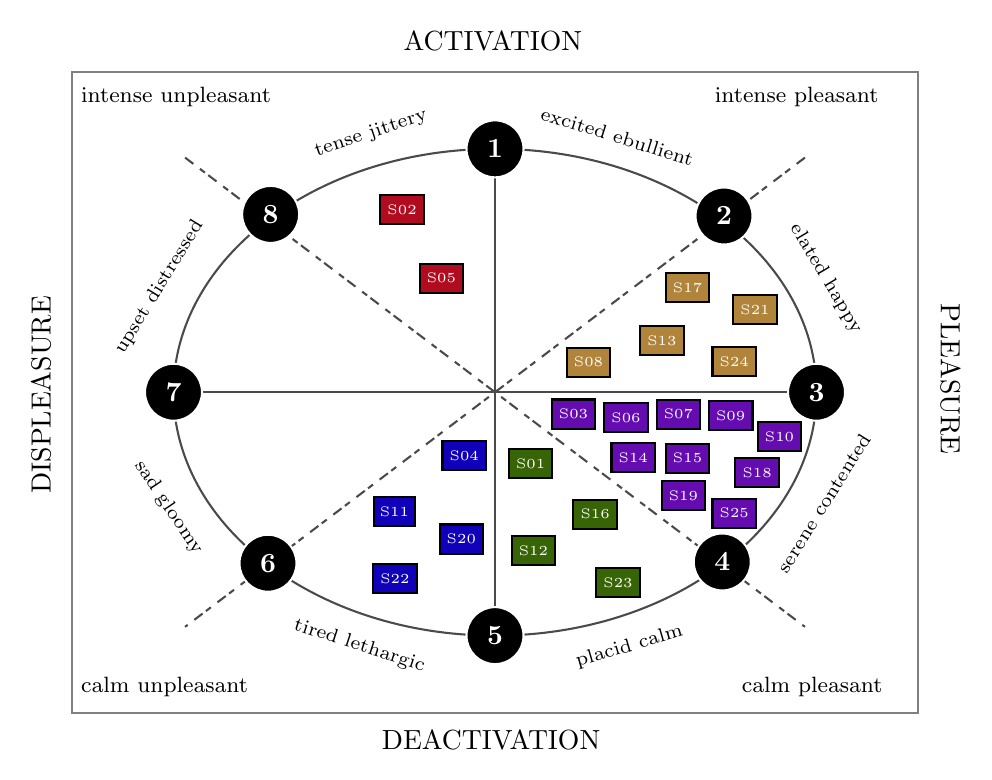
\begin{tikzpicture}[x=0.75pt,y=0.75pt,yscale=-1,xscale=1]
%uncomment if require: \path (0,389); %set diagram left start at 0, and has height of 389

%Flowchart: Or [id:dp3592995680476845] 
\draw  [color={rgb, 255:red, 74; green, 74; blue, 74 }  ,draw opacity=1 ] (182.64,181.1) .. controls (182.64,116.34) and (252,63.84) .. (337.55,63.84) .. controls (423.11,63.84) and (492.46,116.34) .. (492.46,181.1) .. controls (492.46,245.86) and (423.11,298.36) .. (337.55,298.36) .. controls (252,298.36) and (182.64,245.86) .. (182.64,181.1) -- cycle ; \draw  [color={rgb, 255:red, 74; green, 74; blue, 74 }  ,draw opacity=1 ] (182.64,181.1) -- (492.46,181.1) ; \draw  [color={rgb, 255:red, 74; green, 74; blue, 74 }  ,draw opacity=1 ] (337.55,63.84) -- (337.55,298.36) ;
%Straight Lines [id:da30798451784186187] 
\draw [color={rgb, 255:red, 74; green, 74; blue, 74 }  ,draw opacity=1 ] [dash pattern={on 3.75pt off 3pt on 2.25pt off 1.5pt}]  (188.22,68.06) -- (486.88,294.14) ;
%Straight Lines [id:da7804870395610348] 
\draw [color={rgb, 255:red, 74; green, 74; blue, 74 }  ,draw opacity=1 ] [dash pattern={on 3.75pt off 3pt on 2.25pt off 1.5pt}]  (486.88,68.06) -- (188.22,294.14) ;
%Shape: Rectangle [id:dp23344423808181314] 
\draw  [color={rgb, 255:red, 128; green, 128; blue, 128 }  ,draw opacity=1 ] (133.68,26.77) -- (541.42,26.77) -- (541.42,335.43) -- (133.68,335.43) -- cycle ;

% Text Node
\draw  [color={rgb, 255:red, 0; green, 0; blue, 0 }  ,draw opacity=1 ][fill={rgb, 255:red, 176; green, 11; blue, 31 }  ,fill opacity=1 ]  (282.29,86.22) -- (303.29,86.22) -- (303.29,100.22) -- (282.29,100.22) -- cycle  ;
\draw (292.79,93.22) node  [font=\tiny,color={rgb, 255:red, 255; green, 255; blue, 255 }  ,opacity=1 ] [align=left] {S02};
% Text Node
\draw  [color={rgb, 255:red, 0; green, 0; blue, 0 }  ,draw opacity=1 ][fill={rgb, 255:red, 17; green, 0; blue, 185 }  ,fill opacity=1 ]  (279.09,231.64) -- (299.09,231.64) -- (299.09,245.64) -- (279.09,245.64) -- cycle  ;
\draw (289.09,238.64) node  [font=\tiny,color={rgb, 255:red, 255; green, 255; blue, 255 }  ,opacity=1 ] [align=left] {S11};
% Text Node
\draw  [color={rgb, 255:red, 0; green, 0; blue, 0 }  ,draw opacity=1 ][fill={rgb, 255:red, 100; green, 12; blue, 176 }  ,fill opacity=1 ]  (364.87,184.61) -- (385.87,184.61) -- (385.87,198.61) -- (364.87,198.61) -- cycle  ;
\draw (375.37,191.61) node  [font=\tiny,color={rgb, 255:red, 255; green, 255; blue, 255 }  ,opacity=1 ] [align=left] {S03};
% Text Node
\draw  [color={rgb, 255:red, 0; green, 0; blue, 0 }  ,draw opacity=1 ][fill={rgb, 255:red, 176; green, 132; blue, 58 }  ,fill opacity=1 ]  (407.45,149.33) -- (428.45,149.33) -- (428.45,163.33) -- (407.45,163.33) -- cycle  ;
\draw (417.95,156.33) node  [font=\tiny,color={rgb, 255:red, 255; green, 255; blue, 255 }  ,opacity=1 ] [align=left] {S13};
% Text Node
\draw  [color={rgb, 255:red, 0; green, 0; blue, 0 }  ,draw opacity=1 ][fill={rgb, 255:red, 100; green, 12; blue, 176 }  ,fill opacity=1 ]  (440.62,185.49) -- (461.62,185.49) -- (461.62,199.49) -- (440.62,199.49) -- cycle  ;
\draw (451.12,192.49) node  [font=\tiny,color={rgb, 255:red, 255; green, 255; blue, 255 }  ,opacity=1 ] [align=left] {S09};
% Text Node
\draw  [color={rgb, 255:red, 0; green, 0; blue, 0 }  ,draw opacity=1 ][fill={rgb, 255:red, 55; green, 100; blue, 4 }  ,fill opacity=1 ]  (344.22,208.42) -- (365.22,208.42) -- (365.22,222.42) -- (344.22,222.42) -- cycle  ;
\draw (354.72,215.42) node  [font=\tiny,color={rgb, 255:red, 255; green, 255; blue, 255 }  ,opacity=1 ] [align=left] {S01};
% Text Node
\draw  [color={rgb, 255:red, 0; green, 0; blue, 0 }  ,draw opacity=1 ][fill={rgb, 255:red, 176; green, 11; blue, 31 }  ,fill opacity=1 ]  (301.25,119.14) -- (322.25,119.14) -- (322.25,133.14) -- (301.25,133.14) -- cycle  ;
\draw (311.75,126.14) node  [font=\tiny,color={rgb, 255:red, 255; green, 255; blue, 255 }  ,opacity=1 ] [align=left] {S05};
% Text Node
\draw  [color={rgb, 255:red, 0; green, 0; blue, 0 }  ,draw opacity=1 ][fill={rgb, 255:red, 17; green, 0; blue, 185 }  ,fill opacity=1 ]  (312.26,204.61) -- (333.26,204.61) -- (333.26,218.61) -- (312.26,218.61) -- cycle  ;
\draw (322.76,211.61) node  [font=\tiny,color={rgb, 255:red, 255; green, 255; blue, 255 }  ,opacity=1 ] [align=left] {S04};
% Text Node
\draw  [color={rgb, 255:red, 0; green, 0; blue, 0 }  ,draw opacity=1 ][fill={rgb, 255:red, 100; green, 12; blue, 176 }  ,fill opacity=1 ]  (419.83,205.83) -- (440.83,205.83) -- (440.83,219.83) -- (419.83,219.83) -- cycle  ;
\draw (430.33,212.83) node  [font=\tiny,color={rgb, 255:red, 255; green, 255; blue, 255 }  ,opacity=1 ] [align=left] {S15};
% Text Node
\draw  [color={rgb, 255:red, 0; green, 0; blue, 0 }  ,draw opacity=1 ][fill={rgb, 255:red, 100; green, 12; blue, 176 }  ,fill opacity=1 ]  (390.18,186.39) -- (411.18,186.39) -- (411.18,200.39) -- (390.18,200.39) -- cycle  ;
\draw (400.68,193.39) node  [font=\tiny,color={rgb, 255:red, 255; green, 255; blue, 255 }  ,opacity=1 ] [align=left] {S06};
% Text Node
\draw  [color={rgb, 255:red, 0; green, 0; blue, 0 }  ,draw opacity=1 ][fill={rgb, 255:red, 176; green, 132; blue, 58 }  ,fill opacity=1 ]  (372.1,159.61) -- (393.1,159.61) -- (393.1,173.61) -- (372.1,173.61) -- cycle  ;
\draw (382.6,166.61) node  [font=\tiny,color={rgb, 255:red, 255; green, 255; blue, 255 }  ,opacity=1 ] [align=left] {S08};
% Text Node
\draw  [color={rgb, 255:red, 0; green, 0; blue, 0 }  ,draw opacity=1 ][fill={rgb, 255:red, 100; green, 12; blue, 176 }  ,fill opacity=1 ]  (464.11,195.49) -- (485.11,195.49) -- (485.11,209.49) -- (464.11,209.49) -- cycle  ;
\draw (474.61,202.49) node  [font=\tiny,color={rgb, 255:red, 255; green, 255; blue, 255 }  ,opacity=1 ] [align=left] {S10};
% Text Node
\draw  [color={rgb, 255:red, 0; green, 0; blue, 0 }  ,draw opacity=1 ][fill={rgb, 255:red, 100; green, 12; blue, 176 }  ,fill opacity=1 ]  (393.68,205.71) -- (414.68,205.71) -- (414.68,219.71) -- (393.68,219.71) -- cycle  ;
\draw (404.18,212.71) node  [font=\tiny,color={rgb, 255:red, 255; green, 255; blue, 255 }  ,opacity=1 ] [align=left] {S14};
% Text Node
\draw  [color={rgb, 255:red, 0; green, 0; blue, 0 }  ,draw opacity=1 ][fill={rgb, 255:red, 55; green, 100; blue, 4 }  ,fill opacity=1 ]  (345.53,250.28) -- (366.53,250.28) -- (366.53,264.28) -- (345.53,264.28) -- cycle  ;
\draw (356.03,257.28) node  [font=\tiny,color={rgb, 255:red, 255; green, 255; blue, 255 }  ,opacity=1 ] [align=left] {S12};
% Text Node
\draw  [color={rgb, 255:red, 0; green, 0; blue, 0 }  ,draw opacity=1 ][fill={rgb, 255:red, 100; green, 12; blue, 176 }  ,fill opacity=1 ]  (415.44,184.66) -- (436.44,184.66) -- (436.44,198.66) -- (415.44,198.66) -- cycle  ;
\draw (425.94,191.66) node  [font=\tiny,color={rgb, 255:red, 255; green, 255; blue, 255 }  ,opacity=1 ] [align=left] {S07};
% Text Node
\draw  [color={rgb, 255:red, 255; green, 255; blue, 255 }  ,draw opacity=1 ][fill={rgb, 255:red, 0; green, 0; blue, 0 }  ,fill opacity=1 ]  (337.55, 63.84) circle [x radius= 13.73, y radius= 13.73]   ;
\draw (337.55,63.84) node  [font=\normalsize,color={rgb, 255:red, 255; green, 255; blue, 255 }  ,opacity=1 ] [align=left] {\textbf{1}};
% Text Node
\draw  [color={rgb, 255:red, 255; green, 255; blue, 255 }  ,draw opacity=1 ][fill={rgb, 255:red, 0; green, 0; blue, 0 }  ,fill opacity=1 ]  (447.88, 96.18) circle [x radius= 13.73, y radius= 13.73]   ;
\draw (447.88,96.18) node  [font=\normalsize,color={rgb, 255:red, 255; green, 255; blue, 255 }  ,opacity=1 ] [align=left] {\textbf{2}};
% Text Node
\draw  [color={rgb, 255:red, 255; green, 255; blue, 255 }  ,draw opacity=1 ][fill={rgb, 255:red, 0; green, 0; blue, 0 }  ,fill opacity=1 ]  (492.46, 181.1) circle [x radius= 13.73, y radius= 13.73]   ;
\draw (492.46,181.1) node  [font=\normalsize,color={rgb, 255:red, 255; green, 255; blue, 255 }  ,opacity=1 ] [align=left] {\textbf{3}};
% Text Node
\draw  [color={rgb, 255:red, 255; green, 255; blue, 255 }  ,draw opacity=1 ][fill={rgb, 255:red, 0; green, 0; blue, 0 }  ,fill opacity=1 ]  (447.05, 262.88) circle [x radius= 13.73, y radius= 13.73]   ;
\draw (447.05,262.88) node  [font=\normalsize,color={rgb, 255:red, 255; green, 255; blue, 255 }  ,opacity=1 ] [align=left] {\textbf{4}};
% Text Node
\draw  [color={rgb, 255:red, 255; green, 255; blue, 255 }  ,draw opacity=1 ][fill={rgb, 255:red, 0; green, 0; blue, 0 }  ,fill opacity=1 ]  (337.55, 298.36) circle [x radius= 13.73, y radius= 13.73]   ;
\draw (337.55,298.36) node  [font=\normalsize,color={rgb, 255:red, 255; green, 255; blue, 255 }  ,opacity=1 ] [align=left] {\textbf{5}};
% Text Node
\draw  [color={rgb, 255:red, 255; green, 255; blue, 255 }  ,draw opacity=1 ][fill={rgb, 255:red, 0; green, 0; blue, 0 }  ,fill opacity=1 ]  (228.16, 263.49) circle [x radius= 13.73, y radius= 13.73]   ;
\draw (228.16,263.49) node  [font=\normalsize,color={rgb, 255:red, 255; green, 255; blue, 255 }  ,opacity=1 ] [align=left] {\textbf{6}};
% Text Node
\draw  [color={rgb, 255:red, 255; green, 255; blue, 255 }  ,draw opacity=1 ][fill={rgb, 255:red, 0; green, 0; blue, 0 }  ,fill opacity=1 ]  (182.64, 181.1) circle [x radius= 13.73, y radius= 13.73]   ;
\draw (182.64,181.1) node  [font=\normalsize,color={rgb, 255:red, 255; green, 255; blue, 255 }  ,opacity=1 ] [align=left] {\textbf{7}};
% Text Node
\draw  [color={rgb, 255:red, 255; green, 255; blue, 255 }  ,draw opacity=1 ][fill={rgb, 255:red, 0; green, 0; blue, 0 }  ,fill opacity=1 ]  (229.45, 95.43) circle [x radius= 13.73, y radius= 13.73]   ;
\draw (229.45,95.43) node  [font=\normalsize,color={rgb, 255:red, 255; green, 255; blue, 255 }  ,opacity=1 ] [align=left] {\textbf{8}};
% Text Node
\draw (112.89,231.39) node [anchor=north west][inner sep=0.75pt]  [rotate=-270] [align=left] {DISPLEASURE};
% Text Node
\draw (292.08,5.96) node [anchor=north west][inner sep=0.75pt]   [align=left] {ACTIVATION};
% Text Node
\draw (281.58,342.71) node [anchor=north west][inner sep=0.75pt]   [align=left] {DEACTIVATION};
% Text Node
\draw (562.94,136.89) node [anchor=north west][inner sep=0.75pt]  [rotate=-90] [align=left] {PLEASURE};
% Text Node
\draw (150.9,160.23) node [anchor=north west][inner sep=0.75pt]  [font=\scriptsize,rotate=-301.49] [align=left] {upset distressed};
% Text Node
\draw (247.79,60.45) node [anchor=north west][inner sep=0.75pt]  [font=\scriptsize,rotate=-341.6] [align=left] {tense jittery};
% Text Node
\draw (359.94,41.46) node [anchor=north west][inner sep=0.75pt]  [font=\scriptsize,rotate=-17.34] [align=left] {excited ebullient};
% Text Node
\draw (485.75,96.5) node [anchor=north west][inner sep=0.75pt]  [font=\scriptsize,rotate=-59.2] [align=left] {elated happy};
% Text Node
\draw (470.66,265.95) node [anchor=north west][inner sep=0.75pt]  [font=\scriptsize,rotate=-301.93] [align=left] {serene contented};
% Text Node
\draw (373.68,306.2) node [anchor=north west][inner sep=0.75pt]  [font=\scriptsize,rotate=-343.65] [align=left] {placid calm};
% Text Node
\draw (241.21,287.33) node [anchor=north west][inner sep=0.75pt]  [font=\scriptsize,rotate=-18.04] [align=left] {tired lethargic};
% Text Node
\draw (169.56,210.51) node [anchor=north west][inner sep=0.75pt]  [font=\scriptsize,rotate=-56.13] [align=left] {sad gloomy};
% Text Node
\draw (455,317) node [anchor=north west][inner sep=0.75pt]  [font=\footnotesize] [align=left] {calm pleasant};
% Text Node
\draw (136.67,317) node [anchor=north west][inner sep=0.75pt]  [font=\footnotesize] [align=left] {calm unpleasant};
% Text Node
\draw (136.67,32.78) node [anchor=north west][inner sep=0.75pt]  [font=\footnotesize] [align=left] {intense unpleasant};
% Text Node
\draw (442,32.78) node [anchor=north west][inner sep=0.75pt]  [font=\footnotesize] [align=left] {intense pleasant};
% Text Node
\draw  [color={rgb, 255:red, 0; green, 0; blue, 0 }  ,draw opacity=1 ][fill={rgb, 255:red, 55; green, 100; blue, 4 }  ,fill opacity=1 ]  (375.33,232.83) -- (396.33,232.83) -- (396.33,246.83) -- (375.33,246.83) -- cycle  ;
\draw (385.83,239.83) node  [font=\tiny,color={rgb, 255:red, 255; green, 255; blue, 255 }  ,opacity=1 ] [align=left] {S16};
% Text Node
\draw  [color={rgb, 255:red, 0; green, 0; blue, 0 }  ,draw opacity=1 ][fill={rgb, 255:red, 176; green, 132; blue, 58 }  ,fill opacity=1 ]  (419.83,123.83) -- (440.83,123.83) -- (440.83,137.83) -- (419.83,137.83) -- cycle  ;
\draw (430.33,130.83) node  [font=\tiny,color={rgb, 255:red, 255; green, 255; blue, 255 }  ,opacity=1 ] [align=left] {S17};
% Text Node
\draw  [color={rgb, 255:red, 0; green, 0; blue, 0 }  ,draw opacity=1 ][fill={rgb, 255:red, 100; green, 12; blue, 176 }  ,fill opacity=1 ]  (453.33,212.83) -- (474.33,212.83) -- (474.33,226.83) -- (453.33,226.83) -- cycle  ;
\draw (463.83,219.83) node  [font=\tiny,color={rgb, 255:red, 255; green, 255; blue, 255 }  ,opacity=1 ] [align=left] {S18};
% Text Node
\draw  [color={rgb, 255:red, 0; green, 0; blue, 0 }  ,draw opacity=1 ][fill={rgb, 255:red, 100; green, 12; blue, 176 }  ,fill opacity=1 ]  (417.83,223.83) -- (438.83,223.83) -- (438.83,237.83) -- (417.83,237.83) -- cycle  ;
\draw (428.33,230.83) node  [font=\tiny,color={rgb, 255:red, 255; green, 255; blue, 255 }  ,opacity=1 ] [align=left] {S19};
% Text Node
\draw  [color={rgb, 255:red, 0; green, 0; blue, 0 }  ,draw opacity=1 ][fill={rgb, 255:red, 17; green, 0; blue, 185 }  ,fill opacity=1 ]  (310.83,244.83) -- (331.83,244.83) -- (331.83,258.83) -- (310.83,258.83) -- cycle  ;
\draw (321.33,251.83) node  [font=\tiny,color={rgb, 255:red, 255; green, 255; blue, 255 }  ,opacity=1 ] [align=left] {S20};
% Text Node
\draw  [color={rgb, 255:red, 0; green, 0; blue, 0 }  ,draw opacity=1 ][fill={rgb, 255:red, 176; green, 132; blue, 58 }  ,fill opacity=1 ]  (452.33,134.33) -- (473.33,134.33) -- (473.33,148.33) -- (452.33,148.33) -- cycle  ;
\draw (462.83,141.33) node  [font=\tiny,color={rgb, 255:red, 255; green, 255; blue, 255 }  ,opacity=1 ] [align=left] {S21};
% Text Node
\draw  [color={rgb, 255:red, 0; green, 0; blue, 0 }  ,draw opacity=1 ][fill={rgb, 255:red, 17; green, 0; blue, 185 }  ,fill opacity=1 ]  (278.83,263.83) -- (299.83,263.83) -- (299.83,277.83) -- (278.83,277.83) -- cycle  ;
\draw (289.33,270.83) node  [font=\tiny,color={rgb, 255:red, 255; green, 255; blue, 255 }  ,opacity=1 ] [align=left] {S22};
% Text Node
\draw  [color={rgb, 255:red, 0; green, 0; blue, 0 }  ,draw opacity=1 ][fill={rgb, 255:red, 55; green, 100; blue, 4 }  ,fill opacity=1 ]  (386.33,265.83) -- (407.33,265.83) -- (407.33,279.83) -- (386.33,279.83) -- cycle  ;
\draw (396.83,272.83) node  [font=\tiny,color={rgb, 255:red, 255; green, 255; blue, 255 }  ,opacity=1 ] [align=left] {S23};
% Text Node
\draw  [color={rgb, 255:red, 0; green, 0; blue, 0 }  ,draw opacity=1 ][fill={rgb, 255:red, 176; green, 132; blue, 58 }  ,fill opacity=1 ]  (442.33,159.33) -- (463.33,159.33) -- (463.33,173.33) -- (442.33,173.33) -- cycle  ;
\draw (452.83,166.33) node  [font=\tiny,color={rgb, 255:red, 255; green, 255; blue, 255 }  ,opacity=1 ] [align=left] {S24};
% Text Node
\draw  [color={rgb, 255:red, 0; green, 0; blue, 0 }  ,draw opacity=1 ][fill={rgb, 255:red, 100; green, 12; blue, 176 }  ,fill opacity=1 ]  (442.33,232.33) -- (463.33,232.33) -- (463.33,246.33) -- (442.33,246.33) -- cycle  ;
\draw (452.83,239.33) node  [font=\tiny,color={rgb, 255:red, 255; green, 255; blue, 255 }  ,opacity=1 ] [align=left] {S25};


\end{tikzpicture}
